% !TeX spellcheck = en_GB
\documentclass[12pt,fleqn]{article}

\usepackage[danish]{babel}
\usepackage{SpeedyGonzales}
\usepackage{MediocreMike}
%\usepackage{Blastoise}
\usepackage{listings}

\usepackage{float}
\usepackage[caption = false]{subfig}
\title{}
\author{Asger Schultz}
\date{\today}

\fancypagestyle{plain}
{
	\fancyhf{}
	\rfoot{Side \thepage{} af \pageref{LastPage}}
	\renewcommand{\headrulewidth}{0pt}
}
\pagestyle{fancy}
\fancyhf{}
\lhead{Asger Schultz}
\chead{}
\rhead{}
\rfoot{Side \thepage{} af \pageref{LastPage}}

\graphicspath{{Billeder/}}
\linespread{1.15}


%\numberwithin{equation}{section}
%\numberwithin{footnote}{section}
%\numberwithin{figure}{section}
%\numberwithin{table}{section}

\begin{document}

\maketitle
%\thispagestyle{fancy}
%\tableofcontents
--Identifying people from movement curve\\
--Are arm movements of different objects significantly different\\
--Trains, evaluates binary classification tree and 3-nearest neighbour classification to identify people. McNemars test: Find that 3-nearest neighbours is significantly than class. tree and that both are significantly better than baseline.\\
--Using four-way ANOVA, it is found that there is significant difference in arm movements for different experiments.
\tableofcontents
\newpage 


\section{Introduction}

-- Briefly introduce the background \& setting of the problem, as well as the aim of the report. Furthermore, you could give a very short description of the analysis that will be applied.


\section{Data}
The data consists of 16 experiments where ten right-handed people had to move a cylinder over another cylinder.
The size and weight of the cylinders varied over the experiments, and each person had to perform the movement of each experiment 10 times.
Thus, the data was structured in a $ 16\times 10\times 10 $ grid, where the first axis is the experiment, the second the person, and the third the repetition.
For every such repetition, the $ x, y, $ and $ z $ coordinates of the movement where recorded 100 times, such that the data for each repetition was a $ 100\times 3 $ matrix.
The data had been preprocessed such that every curve was of the same length.\\
\\
For our purposes, it was benificial to consider each recording of $ x, y, $ and $ z $ a set of three features, so we ravelled the data such that each repetition had $ 300 $ features with one observation each.
For the first part of the report, we investigated only experiment 4, so we had a total of 100 observations.
The target variable was the person who performed the movement, so the goal of our machine learning models was a 10-class classification.\\
\\
Later, we tested wether or not the experiment had a significant effect.
For this, we ravelled the data points into a vector of length $ 480,000 $, which is explained in more details in section \ref{subsec:expeffect}.

\begin{figure}[H]
		
	\centering
	\subfloat{
		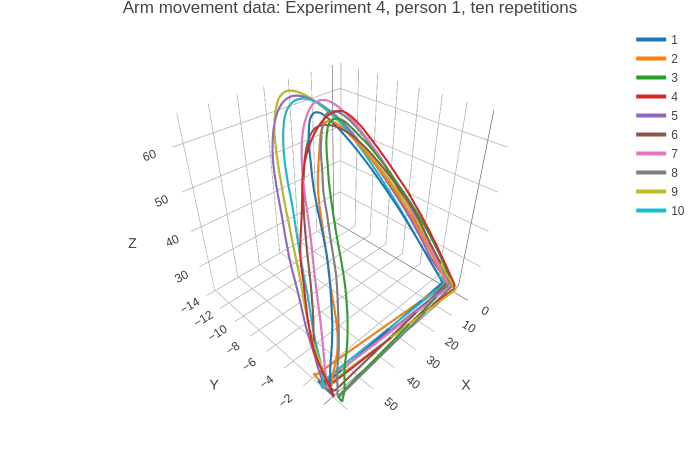
\includegraphics[width=.5\linewidth]{p1_3d_example1}
	}
	\subfloat{
		\centering
		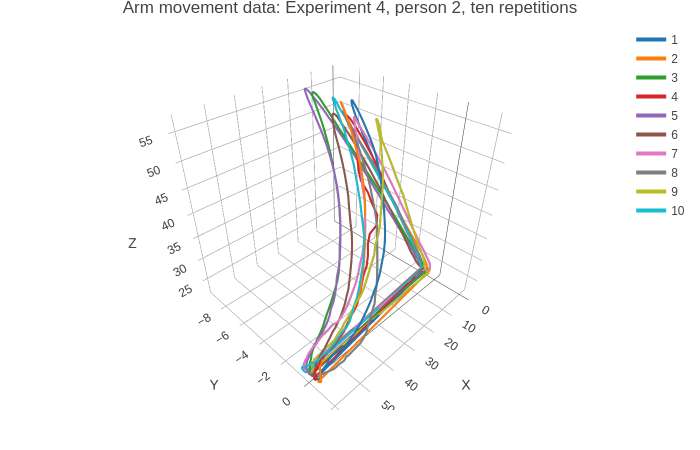
\includegraphics[width=.5\linewidth]{p1_3d_example2}
	}
	\label{fig:trajects}
	\caption{Movies}
\end{figure}


\section{Methods and analysis}


\subsection{Machine Learning Task: Classification}
Two machine learning models were chosen to test on this 300-dimensional 10-class data.
It is noted from initial plots -- fig. \ref{fig:trajects} and fig. \ref{fig:2dtrajects} -- that the effects of different people seem non-linear, such that models that can model nonlinear decision boundaries are considered.
\paragraph{Models} The two chosen models were a binary classification tree and a 3-nearest neighbour classifier. The classification tree used the implementation of Hunt's algorithm of the \texttt{tree} package in \texttt{R} \cite{Tree}. For splitting criterion, the \textit{deviance} is used which is based on minus two times the log likelihood of the data under each model that the split results in \cite{Deviance}.
---Binary classification tree: Hunt's algorithm\\
---3NN: The K value was chosen before based on data dimensionality\\
-- Baseline: 10\pro\\  

\paragraph{Performance evaluation}
--Leave-one-out crossvalidation\\
--McNemar's test\\
-- Note, for McNemar's test: Baseline makes a difference. Was chosen as random guesses, as no single class should be preferred.
\subsection{Test of experiment effect}\label{subsec:expeffect}
Analysis of Variance, or ANOVA, is a method for comparing the means of multiple groups.
This makes it useful for detecting if there is a significant difference between the experiments.
ANOVA works by testing the likelihood of a given mean's distance to the overall mean is due to random variation, which is done using variability decomposition.
We assumed the null hypothesis $ H_0: \mu_1=\mu_2=\ldots=\mu_{16} $.\\
\\
In order to use ANOVA, all the 480,000 data points were ravelled into a vector of the same length.
Four similar vectors where then created for the explanatory variables.
The first contained the coordinates features, such as \texttt{z3} for the third $ z $-value.
The second contained the person, the third the repetition, and the fourth the experiment number.
We then used a linear model with R's \texttt{lm} function followed by \texttt{anova} to perform a four-way ANOVA (given the four explanatory variables).

\section{Results}
\begin{figure}[H]
	\centering
	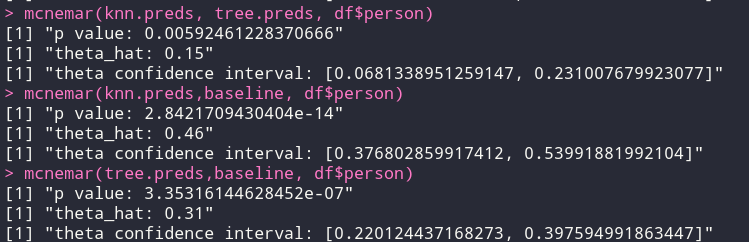
\includegraphics[width=.7\linewidth]{mcnemar_results}
\end{figure}
\begin{figure}[H]
\centering
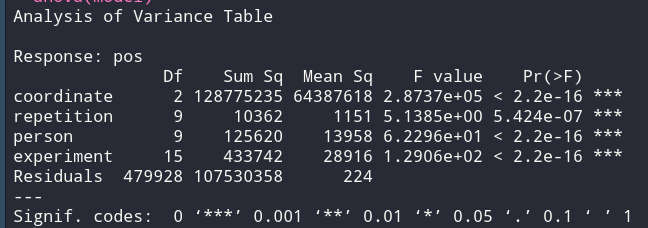
\includegraphics[width=.7\linewidth]{p1_anova}
\end{figure}
\begin{figure}[H]
	\centering
	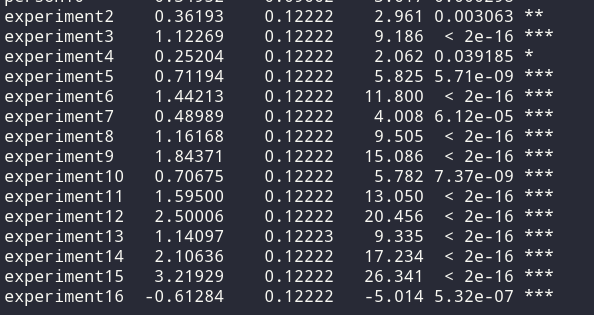
\includegraphics[width=.7\linewidth]{p1_anova_summay}
\end{figure}


Yes, experiment is significant.\\
	
-- All experiments are (at 5\pro) significantly different from the control experiment which has been set to reference

\section{Discussion}
\subsection{Classification of persons}
--Plot: Seems nonlinear (parabolic data)\\
-- Plot: For humans: Easy difference in \(y\)-coordinate between first repetitions of the two initial test subjects.

\subsection{Test of difference in experiments}
-- Expectation: Yes, significant difference as 15 different obtacle avoidance tests + control is considered\\
-- Surprise: Repetition is also significant though\\
-- Which coordinate it is explains the largest part of data variability but experiment no. comes in second\\
-- Low residual variance when compared to within-group variance\\
-- Model assumptions: Plot\\
\begin{thebibliography}{9}
	\bibitem{Tree} Ripley, Brian: "Package ‘tree’", 26/05-19. At: \url{https://cran.r-project.org/web/packages/tree/tree.pdf} (consulted 16/01-20)
	\bibitem{Deviance} Ritschard, Gilbard: "Computing and using the deviance withclassification trees", 01-06. At:
	\url{http://mephisto.unige.ch/pub/publications/gr/ritschard_compstat06.pdf} (consulted 16/01-20)
\end{thebibliography}
\appendix
\section{Appendix: Figures}
\begin{figure}[H]
	
	\centering
	\subfloat{
		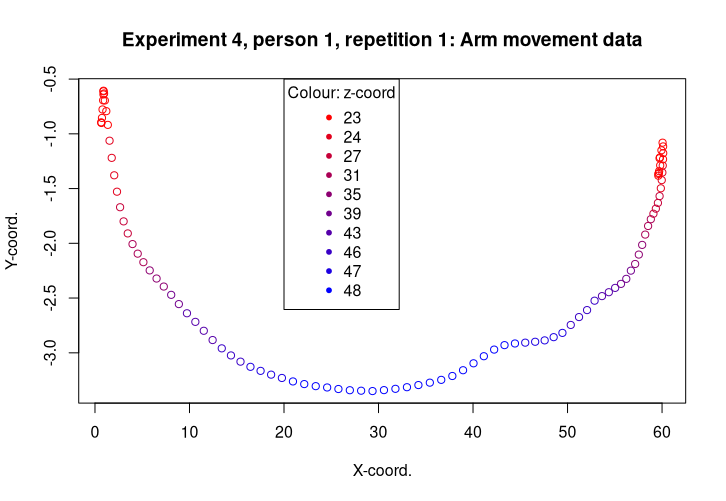
\includegraphics[width=.5\linewidth]{p1_example}
	}
	\subfloat{5
		\centering
		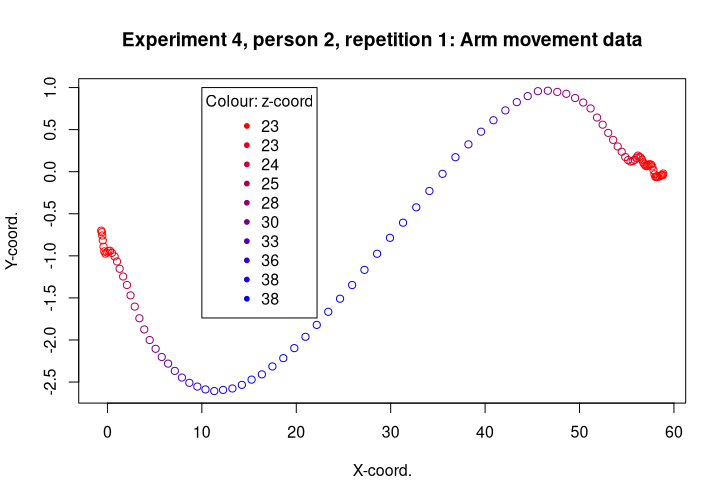
\includegraphics[width=.5\linewidth]{p1_example2}
	}
	\caption{Floats}
	\label{fig:2dtrajects}
\end{figure}


\end{document}

















